\section{Closure Tests}\label{section:star_closure}
In order to  validate the correction procedures, 
closure tests were performed , i.e. full correction procedure was applied to the MC detector-level distributions and the~results were directly compared to the~true-level distributions. Figure~\ref{fig:closure_star} shows closure tests of multiplicity, transverse momentum and pseudorapidity distributions for three ranges of $\xi$, separately.  PYTHIA~8 SD embedding \ac{MC} was used as an~input. In order  to compare  corrected and true-level distributions, the~statistical uncertainties of the~true-level distributions were assumed to be $0$. Due to the method of factorization of the~global efficiency into the product of single-particle efficiencies, a level of non-closure below $5\%$ is typically considered to be sufficient for the validation of the~procedure. However, the~difference between true-level and corrected distributions was taken as a systematic uncertainties.

\begin{figure}[h!]
	\centering
	%\vspace{-2.5cm}
	\begin{subfigure}{.49\textwidth}
		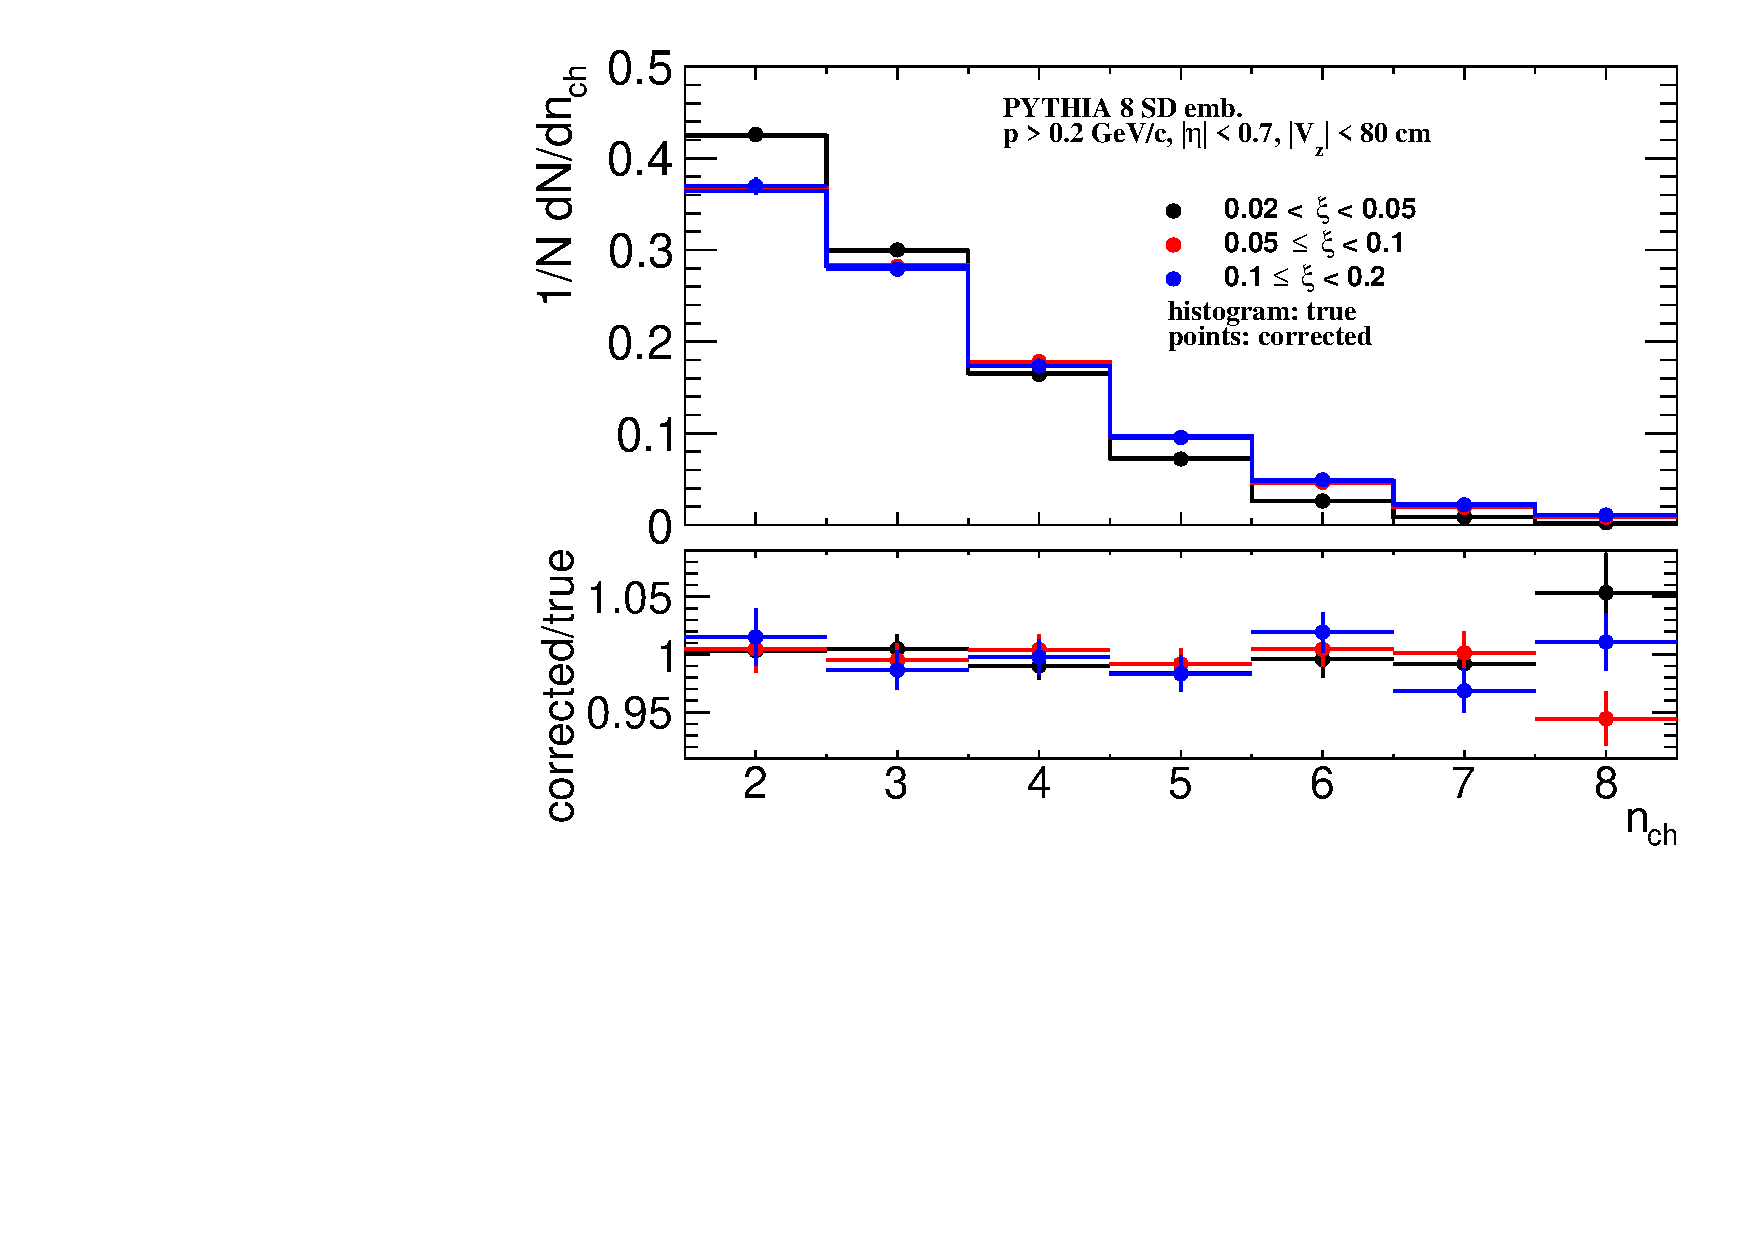
\includegraphics[width=\textwidth,page=1]{chapters/chrgSTAR/img/closure/nch_test.pdf}
	\end{subfigure}
	\begin{subfigure}{.49\textwidth}
		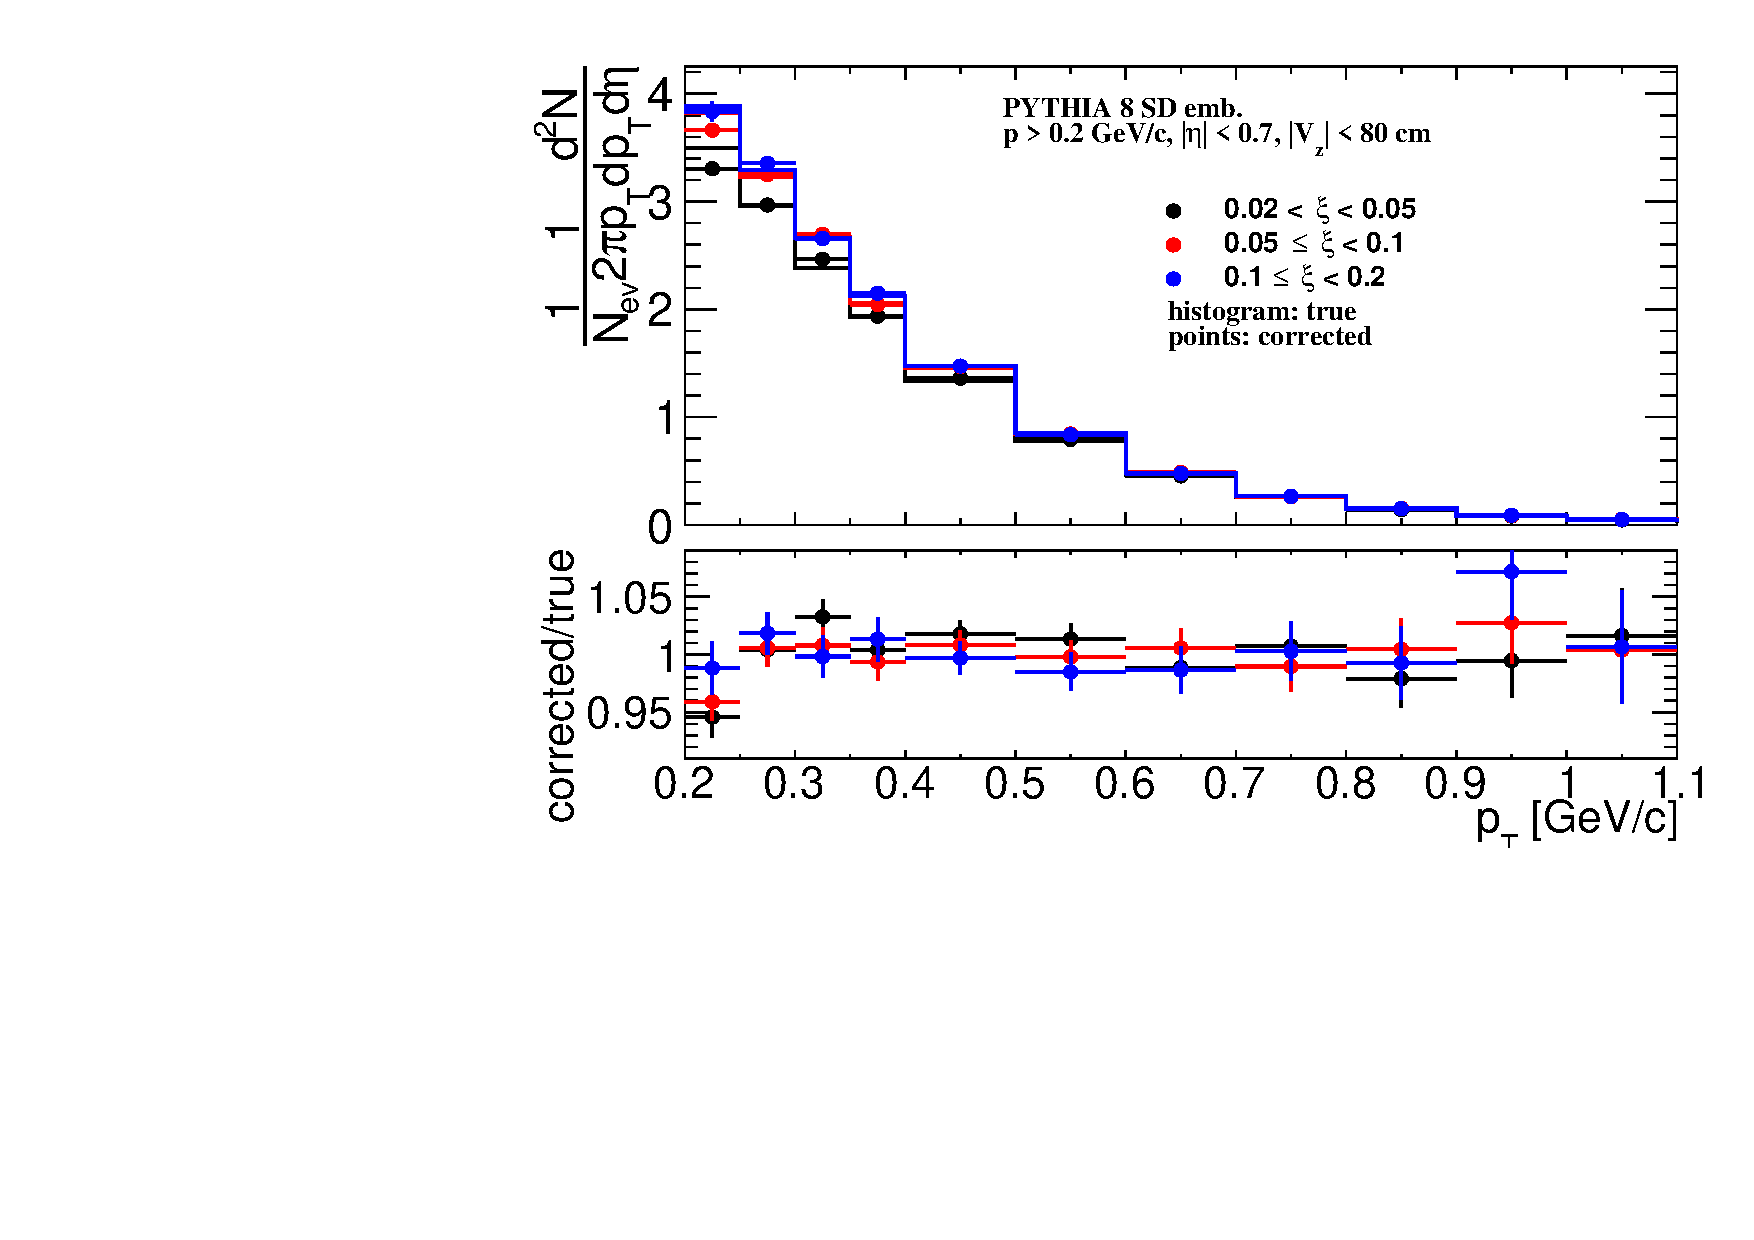
\includegraphics[width=\textwidth,page=1]{chapters/chrgSTAR/img/closure/pt_test.pdf}
	\end{subfigure}
	\begin{subfigure}{.49\textwidth}
		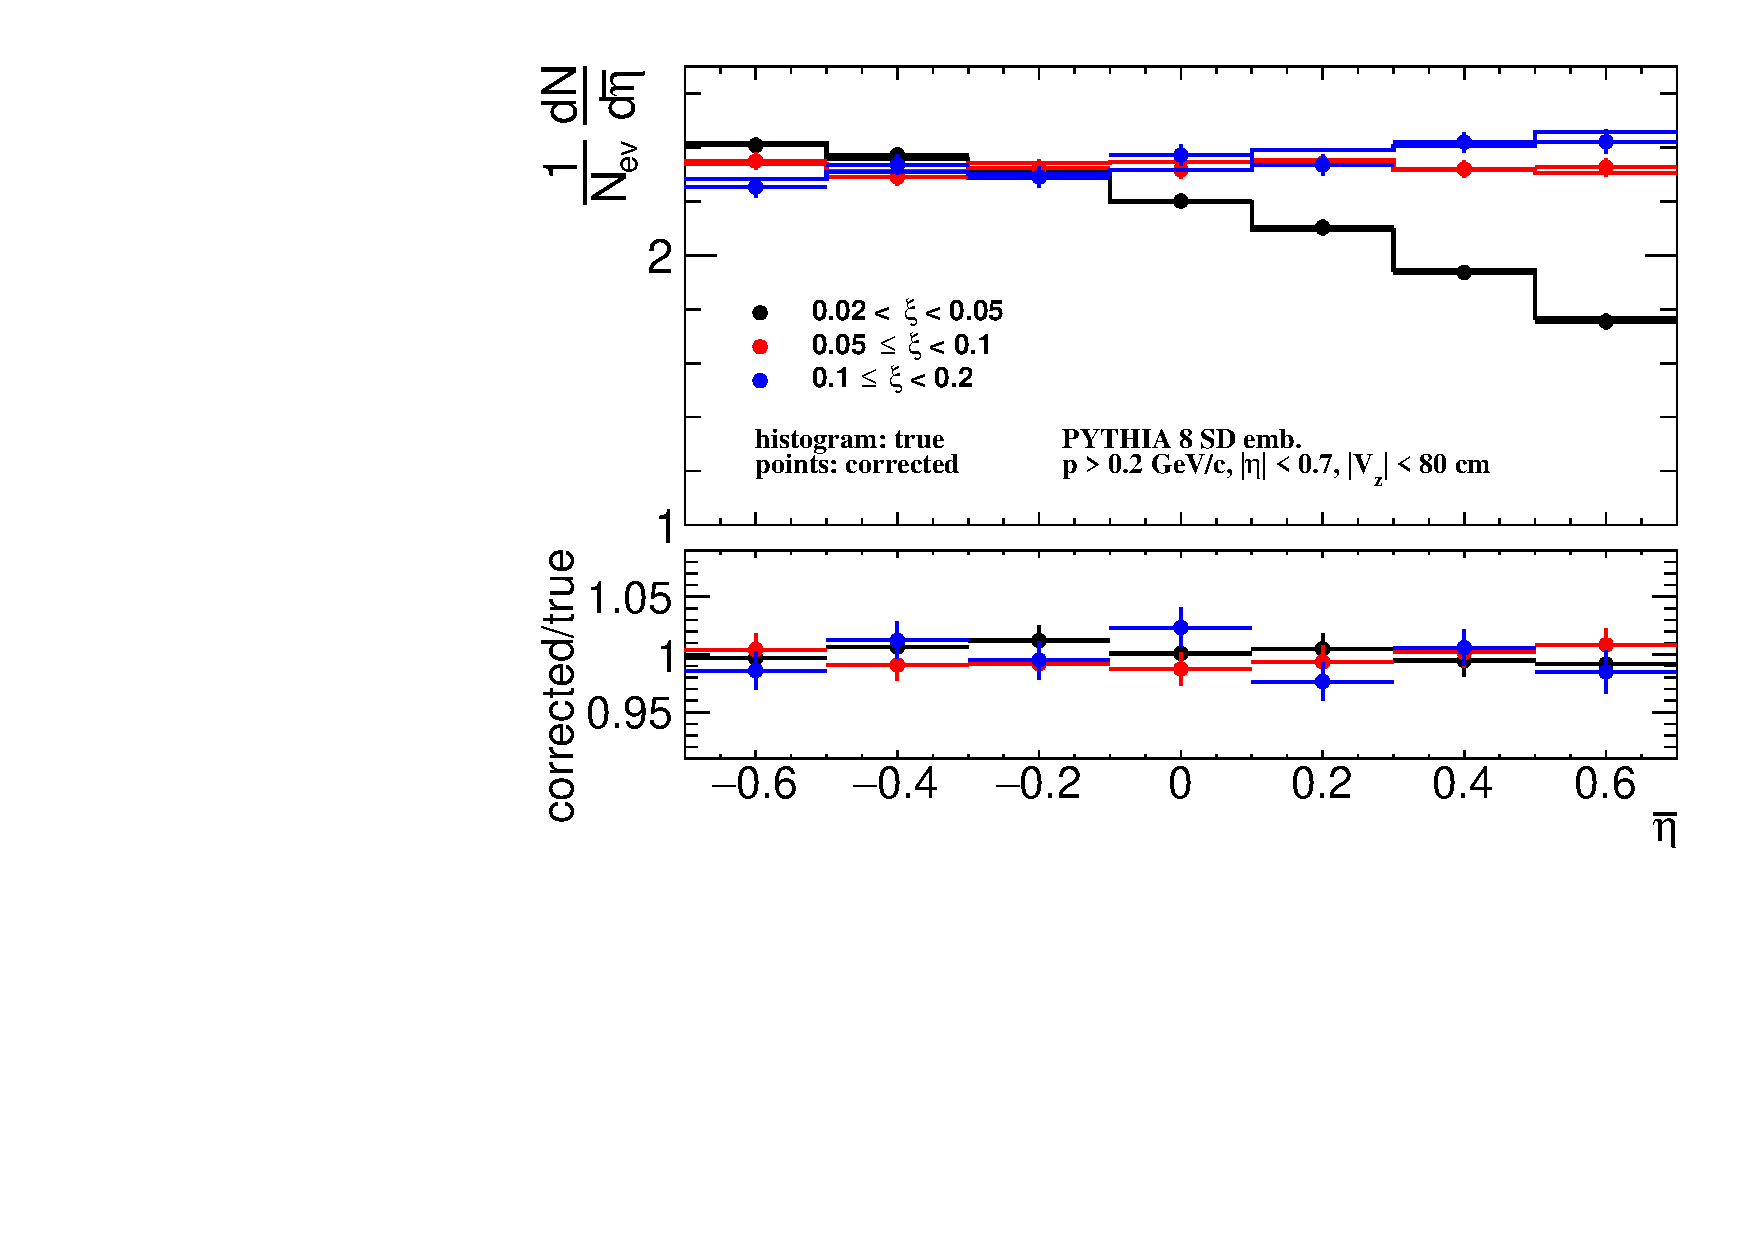
\includegraphics[width=\textwidth,page=1]{chapters/chrgSTAR/img/closure/eta_test.pdf}
	\end{subfigure}
	\begin{minipage}{.49\textwidth}
		\caption{Closure tests of (top left) multiplicity, (top right) transverse momentum and (bottom) psuedorapidity distributions for three ranges of $\xi$ using PYTHIA~8 SD embedding MC.}
		\label{fig:closure_star}
	\end{minipage}
	
	%\vspace{-1.5cm}
	%\vspace{-2cm}
\end{figure}


 
